
\section*{\centering Основные результаты и выводы}
\addcontentsline{toc}{chapter}{Основные результаты и выводы}


\begin{figure}
\center{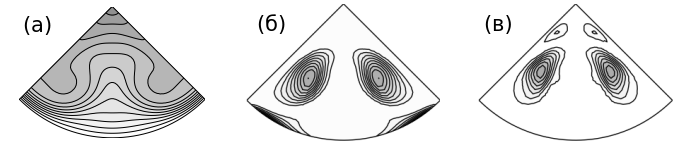
\includegraphics[width=1\linewidth]{ub_cs.png}}
\caption{Поле скорости решения с верхней ветви}
\label{ub_cs_pic}
\end{figure}

\noindent $1.$ Рассчитан и исследован модельный порыв --- условно-периодическое решение уравнений Навье-Стокса с пространственно-локализованной структурой, являющееся предельным состоянием решения, эволюционирующего на сепаратрисе, разделяющей в фазовом пространстве области притяжения решений, соответствующих ламинарному и турбулентному режимам течения. Это решение воспроизводит характерные особенности турбулентного порыва, но имеет более простое временное поведение, что позволяет выполнить его детальное исследование. Определены основные элементы механизма поддержания колебаний в модельном порыве. Его поле скорости представляется в виде суперпозиции средней и пульсационной составляющих. Характерной особенностью среднего течения является наличие вытянутых вдоль потока полос повышенной и пониженной скорости. Пульсации возникают в результате линейной неустойчивости среднего течения в областях между соседними полосами. В этих областях находятся точки перегиба, если рассматривать среднее течение как функцию угловой переменной, что позволяет связать механизм образования колебаний с неустойчивостью струйного течения с токами перегиба. Продольная неоднородность среднего течения не является необходимым условием возникновения пульсаций. Угловую неоднородность среднего течения поддерживают продольные вихри, перемещающие жидкость в нормальной к основному потоку плоскости. Продольные вихри, в свою очередь, формируются в результате нелинейного взаимодействия пульсаций. Таким образом, можно говорить о цикле поддержания колебаний. 

\noindent $2.$ Обнаружен нелинейный механизм поддержания продольных вихрей, вызывающих полосчатое искажение в распределении продольной скорости. Существование продольных вихрей поддерживается нелинейным взаимодействием пульсаций продольной скорости и пульсаций продольной завихренности. Пульсации продольной завихренности образуются за счет сжатия и растяжения существующих в среднем течении вихревых трубок пульсациями продольной скорости, что обеспечивает необходимую для поддержания продольных вихрей согласованность фаз между этими пульсациями. 

\noindent $3.$ Рассчитано и исследовано семейство условно-периодических решений уравнений Навье-Стокса с пространственно локализованной структурой, полученное продолжением решения, соответствующего модельному порыву, по числу Рейнольдса. Также рассчитано и исследовано три семейства решений, имеющих вид бегущих волн. Одно семейство описывает течение в круглой трубе и два --- в плоском канале. Механизм поддержания колебаний во всех исследованных решениях аналогичен найденному в модельном порыве, что подтверждает его универсальность. 
